\documentclass[10pt,conference]{IEEEtran}
%\documentclass[a4paper,12pt]{article}

\usepackage{cite,latexsym,times,epsf,amsmath,amssymb,amsfonts,graphicx}
\usepackage{epstopdf}
\usepackage{graphicx}
\usepackage{subfigure}
\usepackage{multirow}
\usepackage{algorithmic}
\usepackage{algorithm}
\usepackage{verbatim}
\renewcommand{\algorithmicrequire}{\textbf{Input:}}
\renewcommand{\algorithmicensure}{\textbf{Output:}}
\renewcommand{\baselinestretch}{0.94}
\setlength{\textfloatsep}{0pt}% Remove \textfloatsep

\begin{document}
\title{Leveraging Diverse Propagation and Context for Multi-Modal Vehicular Applications}
\author{Pengfei Cui, Hui Liu, Jialin He, Onur Altintas, Rama Vuyyuru, Dinesh Rajan, and Joseph Camp \\
%Department of Electrical Engineering,\\ Southern Methodist University (SMU), Dallas, TX \\
%\{camp\}@smu.edu  \\
}
%\documentclass[10pt]{article}

%\usepackage{xkvltxp}
%\usepackage{fixme}


\maketitle


\begin{abstract} 

The emergence of the reapportioned white space bands for data usage will fuel the already
increasing frequency band diversity of today's wireless hardware. As a result, many
existing multi-channel and/or multi-band adaptation schemes will become more important.
Many of these works have considered the capacity and channel activity of these channels,
but have not distinguished between the propagation characteristics that occur when considering
a difference in frequency of multiple GHz and the resulting effect in various environments.
In this paper, we leverage the contextual information and propagation diversity to enable
adaptation across a number of frequency bands from 700 MHz to 5.8 GHz.  To do so, we
perform a number of experiments in a vehicular environment using a campus bus.  With a
model based on a Support Vector Machine (SVM) and an in-situ training set, we can predict
the throughput on a free channel.  We can then consider the activity level per band to 
compute the net throughput we should expect on a given band to guide our adaptation protocol.  
In the field, we exploit the propagation differences experience per band to show that training on a repeatable 
route can yield vast performance improvements from prior schemes.  We show that minimal  
amounts of training can provide such improvements and that a simple scheme that can allow
multiband adaptation gains when there is insufficient levels of training.


%Probably at this time we could not employ the bus doing the experiments.

%Unused spectrum whitespaces in the currently underutilized analog TV bands are able to exploit for future wireless networks. There are potential room for performance improvement of wireless communication in throughput, power consumption and link fairness extending wireless to these bands. Previous methods are focused on channel adaptation across multiple channels in one band without considering the propogation and other characters among different bands. In this work, we employ the propogation difference for performance prediction of multiband adaptation. To identify the crowded level,we involve an activity level of networks based on the statistics information during a time slot to make the prediction more accuracy. The amount of context information required for multiband adaptation and the influerence of window size for activity level are evaluated in this paper. We conduct indoor and in-field experiments to validate our method. The experimental results demonstrate that our method is able to achieve as ... 


\end{abstract}



\let\thefootnote\relax\footnotetext{P. Cui, H. Liu, J. He, D. Rajan, and J. Camp are with Southern Methodist University, Dallas, TX.
O. Altintas is with Toyota InfoTechnology Center, Co. Ltd., Tokyo, Japan. R. Vuyyuru is with Toyota InfoTechnology Center, U.S.A. Inc., Mountain View, CA.  The SMU authors were supported on this work by NSF grants CNS-0958436, CNS-1040429, and CNS-1150215.}

%\section{Contributions}
\label{sec:introduction}


The main contributions of our work are as follows:
\begin{itemize}

\item Understand the role of propagation on multiband information via the use of context information.
\item Evaluating the amount of training necessary for gains in multiband adaptation.
\item Leverage path loss estimation in a particular environment when there is insufficient contextual training
to produce gains.
\item Verify the framework through emulated, indoor, and in-field experimental trials.
\end{itemize}






\section{Introduction}
\label{sec:introduction}


%Background
%Worldwide governments and societies are active to achieve road safety and travel comfort of drivers and passengers.
Drivers and passengers around the world could utilize a wide array of vehicular applications ranging from real-time traffic monitoring and
safety applications to various {\it infotainment} applications.
%spanning news, weather, audio, and video streams.  
However, the continuous use of such applications is limited due to the challenge of transmitting over 
highly-dynamic vehicular wireless channels. 
In such networks, the increasing availability of different 
frequency bands with correspondingly diverse propagation characteristics could allow flexibility and 
robustness of vehicular links. Even with spectral flexibility, links are extremely tenuous, 
demanding instantaneous decisions to remain connected, motivating an algorithm that
can find the appropriate frequency band quickly and according to the current environmental context.

Cognitive radio mechanisms which interleave channel accesses also motivate the frequency
band selection problem of finding the optimal spectrum on which to 
transmit~\cite{ghasemi2008spectrum}.
%Furthermore, in existing systems, there are a number of different technologies from which to choose and the demand of
% integrating the advantages of multiple protocol is presented as Heterogeneous Wireless Networks has opening topics related to band selection~\cite{hossain2010vehicular}.
Prior work has considered a number of challenges in
leveraging white space frequencies including spectrum sensing, frequency-agile operation,
geolocation, solving stringent spectral mask requirements, and providing reliable service
in unlicensed and dynamically changing spectrum~\cite{shellhammer2009technical}. In particular, there has recently been an acceleration
in spectrum sensing work~\cite{rayanchu2011fluid, kim1996pulse,cabric2004implementation}. Based on 
these works, protocols have been built for multi-channel and/or multiband wireless operation~\cite{MOAR,
raychaudhuri2003spectrum,sabharwal2007opportunistic}.  Other works have presented methods for searching for the most efficient 
transmission channel~\cite{mo2005comparison}, discovering channel information~\cite{rayanchu2011fluid, sabharwal2007opportunistic}, and estimating 
channel quality~\cite{MOAR}.
Finally, the emergence of a number of diverse sensors on a vehicle motivates work
on heterogeneous wireless networks, which have different frequency bands {\it and}
technologies~\cite{hossain2010vehicular}. Thus, the various communication 
standards have diverse throughput capacity, allowing the choice of technology 
to possibly usurp frequency band decisions. For example, an 802.11n link at 5.8 
GHz with high levels of loss
might still be a better choice than a Bluetooth link at 2.4 GHz with little loss
due to the discrepancy of hundreds of Mbps in throughput capacity.
%To consider the choice of frequency band, band selection problem for htereogeneous wireless networks should be researched under the same protocol, which make it similar to our problem~\cite{hossain2010vehicular}.
%Add heterogeneous and cognitive radio
%Research of heterogeneous wireless networks has been done for these purpose in Roadside-to-Vehicle and Vehicle-to-Vehicle.\cite{hossain2010vehicular}.
%the understanding of primary/secondary users adaptation\cite{cordeiro2007c}, combining multiple devices for vehicle~\cite{hossain2010vehicular}.

However, for the purposes of this work, we assume the underlying technology is the same to evaluate the choice of frequency band.
While these works have considered spectral activity and developing protocols and algorithms to 
find spectral holes, less of a focus has been on coupling such information with historical performance in a given 
propagation environment.
In this paper, 
we develop multiband adaptation protocols which couple the prior knowledge of in-situ performance of various bands with the instantaneous knowledge of 
spectral activity, SNR, and current location of each band to arrive at a decision on the optimal band to transmit. To do so, we use an
off-the-shelf platform that allows direct comparison and simultaneous experimentation across four different wireless
frequency bands from 450 MHz to 5.8 GHz with the same physical
and media access layers. 
%changes that frequency differences of hundreds of MHz to GHz could have on the band %decision. Moreover, it is well known that propagation greatly depends on the environment %in operation~\cite{rappaport}.  Thus, knowledge of the environment in operation could %allow the relationship between received power differences across multiple frequency bands %to have much greater accuracy.  

%Contributions  fixme
The main contributions of our work are as follows:
\begin{itemize}
\item We first develop a framework for multiband adaptation using both historical information and instantaneous measurements. This framework is broad enough to study adaptation across licensed and unlicensed bands, including white space frequency bands.  

\item We propose two different machine-learning-based multiband adaptation algorithms. The 
first machine learning algorithm, referred to as the \emph{Location-based 
Look-up Algorithm}, 
is based on the idea of $k$-nearest-neighbor classification. The second machine-learning-based 
algorithm uses \emph{decision trees} for classification. 
For comparison, we also create two baseline adaptation algorithms which attempt to make the optimal band selection based on only: (i.)~historical 
performance data, and (ii.)~instantaneous SNR measurements across 
various bands. 

%We consider four different algorithms for comparison.  First, we consider a scheme
%in which the throughput is achieved on an emulated channel for
%the current received signal level. We then adjust the predicted best band choice according to the current activity
%level (real-time information). 
%Second, we consider an approach based on machine learning which
%considers prior throughput for a given received signal and activity level
%combination.  
%Third, we build a scheme which include the prior relationship of throughput, received signal level and context information in an look up table for repeatable travel in an area.
%Fourth, we split the area to different regions and apply machine learning in each region to get the property band selection.

%earning in addition to the received signal and activity level.
%Third, we consider a second machine learning approach which considers user
%location in addition to the received signal and activity level.

\item We perform extensive outdoor V-2-V experiments to evaluate the proposed algorithms.
Our results indicate that the proposed machine learning based algorithms improve
throughput by up to $49.3\%$ over these baseline methods.

\end{itemize}



%The remainder of this paper is organized as follows. In Section II, we present the multiband adaptation problem and proposed algorithms. Section III discusses experimental evaluation of the multiband algorithms. We conclude in Section IV.


\section{Multiband Adaptation}
\label{sec:model}
In this section, we first focus on the problem formulation for multiband 
adaptation in vehicular wireless links and introduce the context information 
that we use. Based on the analysis of existing problems, we discuss two 
baseline methods for comparison and propose two machine-learning-based 
multiband adaptation algorithms for vehicular channels.

\subsection{Problem Formulation}
The problem we are going to resolve is to find a band has the best throughput in multiple available options as:
\begin{align}
\label{eqn:estimation}
f: (v_{tx}, v_{rx},  P_R^1,..., P_R^n, B^1, ..., B^n,P_N^1,..., P_N^n,) \rightarrow b_{best}
 \end{align}
where $v_{tx}$ and $v_{rx}$ are the velocity of the transmitter and the receiver, 
$P_R^i$ is the received power, $P_N^i$ is the no-802.11 interference signal level and
 %Why we use context information 
$B^i$ is the \emph{busy time}.


To represent the unusable level of the channel, we define \emph{busy time}, $B$,
as the percentage of time when the channel is occupied by 
all competing sources $x_j ( j = 1, 2, 3, ...)$ other than the intended transmitter $y$. 
For 802.11-based transmissions, the busy time on band $i$ could be defined as:
\begin{equation}
\label{eqn:80211activity}
B^i = \frac{\sum_j{\sum_k{\frac{L_k^{x_j}}{R_k^{x_j}}}}}{\sum_k{\frac{L_k^y}{R_k^y}}+\sum_j{\sum_k{\frac{L_k^{x_j}}{R_k^{x_j}}}}+S\sigma}
\end{equation}
where $L$ and $R$ represent the length of packet in bits and the data
rate that packet is transmitted, respectively, for all external sources $x_i$
as compared to the idle slots $S$ times the slot duration $\sigma$ and
the packets from the intended transmitter $y$. When considering the level of
activity of non-802.11 users (e.g., the bands currently licensed to TV 
and other non-802.11 devices), whether the signal level from these
competing sources reaches a level to disrupt communication at the receiver
would define a similar notion of busy time. However, since this depends
on the environment, hardware, coding, and modulation level, we use
the received signal level from non-802.11 interference sources $P_N^i$ 
on band $i$ as an input to our algorithms in various forms as shown 
in~(\ref{eqn:estimation}).

The existing patten embedded in the performance of different bands and 
collected context information e.g. $v_{tx}$, $v_{rx}$, $B_i$, $P_N^i$, $P_R^i$ 
and location information, $g$, could be extracted and help make decisions
for multiband adaptation in a similar context~\cite{meikle2012global} .
%can be used by people tending to have repeatable patterns
%~\cite{meikle2012global} and we could improve the performance with each trip 
%to the region if we could passively observe context along this repeatable 
%pattern. The variables used in each algorithm will be explained for each algorithm 
%later. 

\subsection{Multiband Adaptation Algorithms}
%2 baseline methods: 
%1. band selection based on identifying the the most common class, 
%2. SNR-based band selection
In order to evaluate the proposed multiband adaptation algorithms, 
we construct two simple multiband adaptation methods: (1) We search the
most commonly selected band as the best band in the historical data
and configure the most common band as the final decision. (2) For each band, we build 
a lookup table for throughput $T_{ideal}$ in the ideal channel given $RSSI$ and obtain 
the best band according to following:
\begin{align}
&\max_i T_{ideal}^i\times(1-B^i),
\label{eq:baseline2}
\end{align}
The throughput $T_{ideal}$ is measured with Azimuth ACE-MX channel emulator~\cite{AzimuthACE}. 
The details of system setup and data collection are discussed in Section~\ref{sec:experiment design}. 

Machine learning has been introduced as an important tool in wireless communication
~\cite{haykin2005cognitive}. When the user enters an area, the machine
learning algorithm can learn from the historical data and train a mapping 
function to select the potential optimal band given the input, e.g. RSSI, velocity 
and activity level. We propose two multiband adaptation algorithms based on
two machine learning methods: the k-nearest neighbor (KNN) and the decision tree.

%2 machine learning methods: 
%1. modified KNN, 

{\bf Location based Look-up Algorithm.} KNN is a machine learning method
based on searching closest training data points in the feature space and various
modified versions has been applied successfully for classification~\cite{zhang2006svm}.
In the Location based Look up Algorithm, we search the closest neighbors of 
a testing points by using the parameter one by one in the input set. The 
performance of the found training data points is averaged in each band. Then
the band with the highest throughput performance is selected as the $b_best$.
The Location based look-up algorithm involves the geographic information 
for the band selection comparing with \emph{Machine Learning Algorithm}. 
The process of this algorithm is presented as \ref{algorithms: Location}:
	  \begin{algorithm}
	  \caption{Location based Look-up Algorithm}
	  \label{algorithms: Location}
	  \begin{algorithmic}[1]
	  \REQUIRE  ~~\\
		  $P_R^i \in \{P_R^1,P_R^2 \dots,P_R^n\}$;\\
		  $B^i \in \{B^1,B^2, \dots, B^n\}$;\\
		  $P_N^i \in \{P_N^1,P_N^2 \dots,P_N^n\}$;\\
		  $v_tx$\\
		  $g$: Location Information of Multi-band node\\
		  $Thr_{Area}$: Threshold of a Location\\
		  $Thr_{RSSI}$: Threshold of RSSI\\
		  $Thr_{Velocity}$: Threshold of Velocity\\
		  $Thr_{A Area}$: Threshold of Data Amount for Location\\
		  $Thr_{A RSSI}$: Threshold of Data Amount for RSSI\\
		  $Thr_{A Non 802.11 SI}$: Threshold of Data Amount for Non 802.11 Interference\\
		  $Thr_{A Velocity}$: Threshold of Data Amount for Velocity\\
		  $D^i \in \{D_1,D_2,\dots,D_n\}$: Historical Look up data
\ENSURE ~~\\    
$b_{best}$:Optimal transmission band
\FOR    {$i<=n$}
\STATE Initialize \emph{$Data_{Location},Data_{RSSI},Data_{Velocity}$} to zero matrix;
\WHILE {$Amount(Data_{Location,i})<Thr_{A Area}$}
\STATE $Data_{Location,i} \leftarrow f_{Lookup}(D^i,g,Thr_{Area})$: Find data in $D^i$ whose distance less than $Thr_{Area}$;
\STATE $Thr_{Area}=Thr_{Area} \times 1.1$;
\ENDWHILE

\WHILE {$Amount(Data_{RSSI,i})<Thr_{A RSSI}$}
\STATE $Data_{RSSI,i} \leftarrow f_{Look-up}(D_{Location,i},P_R^i,Thr_{RSSI})$: Find data in $D_{Location}$ the RSSI similar to $P_R^i$ in range $Thr_{RSSI}$;
\STATE $Thr_{RSSI}=Thr_{RSSI} \times 1.1$;
\ENDWHILE

\WHILE {$Amount(Data_{P_N,i})<Thr_{A Non 802.11 SI}$}
\STATE $Data_{RSSI,i} \leftarrow f_{Look-up}(D_{Location,i},P_N^i,Thr_{RSSI})$: Find data in $D_{Location}$ the RSSI similar to $P_N^i$ in range $Thr_{RSSI}$;
\STATE $Thr_{A Non 802.11 SI}=Thr_{A Non 802.11 SI} \times 1.1$;
\ENDWHILE

\WHILE {$Amount(Data_{Velocity,i})<Thr_{A Velocity}$}
\STATE $Data_{Velocity,i} \leftarrow f_{Lookup}(D_{RSSI,i},v_tx,Thr_{Velocity})$: Find data in $D_{RSSI}$ the RSSI similar to $v_tx$ in range $Thr_{RSSI}$;
\STATE $Thr_{Velocity}=Thr_{Velocity} \times 1.1$;
\ENDWHILE \\

\STATE $Tpt_{L,i}=avr(Data_{Velocity,i})$;
\STATE  $Tpt_{e,i}=Tpt_{L,i}\times(1-b_i)$;
\ENDFOR \\  
\STATE $b^*=Max\{Tpt_{e,1},Tpt_{e,1},\dots,Tpt_{e,n}\}$;\\
\end{algorithmic}
\end{algorithm}

For \emph{Location Based Look up Algorithm}, $B_i$ is the \emph{busy time}; $v_i$ 
is the \emph{Velocity} of each band and $r_i$ is the \emph{RSSI} of each band. 
Context information $c$ involves $g$, $v$, and $B^i$. In the 
process of each data point, we have $4$ looking up process to narrow down the data 
points which is similar to the testing data point. First, we find an amount of 
historical data which is near the testing data in a distance range, if the amount of 
historical data which qualify the requirement, we increase the distance range; then we 
narrow the data in the previous looking up qualify the data has similar RSSI in a 
range, if the amount is less than a threshold $Thr_{RSSI}$, the RSSI range will be 
increased; the process is repeated for non 802.11 interference signal and velocity.
At last, the average throughput of the most similar data will be adjust of the 802.11 
\emph{busy time} and tell the best band.

%2. region-based C4.5 (different region sizes)
{\bf Region-based Decision Tree algorithm.} Decision trees are one kind of the most 
widely used machine learning 
algorithms according to its low complexity and stable performance~\cite{banfield2007}.
The decision tree can model the relationship in the training data between the context 
information and the optimal band as a set of tree-like deduction structure. Before 
implementing the training process, we prepare a training set including a group of 
training data points as $\{v_{tx}, v_{rx}, P_R^1, ..., P_R^n,  B^1, ..., B^n, P_N^1, 
..., P_N^n, b_{best}\}$ based on the collected measurements. We obtain $b_best$ by comparing
the throughput performance of all available bands and selecting the band with the highest 
throughput. We choose C4.5 algorithm~\cite{hall2009weka}, an information entropy gain based
and widely used algorithm to build the decision tree used in our system. At each intermediate
node, the learning algorithm calculate the information entropy gain of splitting the rest 
training data points based on each parameter in the input set, e.g. RSSI, velocity or 
activity level. Then it compare and select the parameter with the highest entropy gain
to decide the test condition at each intermediate node until all training data points are
classified. The leaf node indicates the optimal band for prediction in our application
Then the trained decision structure is integrated into the transmission system. With the
collected context information fed into, the decision structure can suggest the potential 
band with the best throughput performance for transmission. 

The relationship between the context information and the best band could be changed at 
different locations because of different propagation environment. To reduce the interference
of training data from different locations, we split the routing of the 
vehicles into several regions and implement the training process based on the historical 
data collected in each region. Then trained decision structure is integrated in our system 
for multiband adaptation in each region. The granularity of region division is one parameter
that affect the training set as well as the performance of the resulting decision tree. We 
evaluate granularity of division in Section~\ref{sec:experiment design}.

\section{Experimental Analysis for Prediction Algorithms}
\label{sec:experiment design}

As discussed in Section 3, some algorithms are more appropriate in certain 
scenarios. To study these algorithmic differences, we have developed indoor 
and in-field experiments on an off-the-shelf wireless platform.
%Testbed and emulator Platform
To ensure the results are broadly applicable, we employ a Linux-based 
802.11 testbed~\cite{Openwrt}. The platform includes a Gateworks 2358 
motherboard with Ubiquiti XR series radios (XR9 at 900 MHz, XR2 at 2.4 GHz, 
XR5 at 5.2 GHz) as well as a DoodleLabs DL475 radio at 
450 MHz~\cite{Gateworks,Ubnt}.  Another instrument involved in the 
experimentation is an Azimuth ACE-MX channel emulator, allowing 
controllable propagation and fading characteristics with a broad range of 
industry-standard channel models from 450 MHz to 5.9 GHz~\cite{AzimuthACE}. 

%context information experiments
\subsection{In-lab Experiments for Radio Characterization}
\label{subsec:ichannel}
To establish an SNR to throughput relationship for the \emph{SNR-based 
Throughput Look-up Algorithm}, we use an experimental setup where two 
wireless nodes communicate across repeatable emulated channels generated 
by Azimuth ACE-MX channel emulator (Fig.~\ref{fig:in-door experiment}). For a given band and card, we measure
the throughput of a fully-backlogged UDP flow using the {\it iperf} 
traffic generator. We use constant attenuation over an idealized
channel condition (i.e., a bypass channel) and repeat the experiment to
produce various RSSI values.
Despite the same physical and media access layers of the radios, there are
slight differences in the throughput achieved per radio at the same attenuation
level.  Thus, we normalize these throughput values to have the same maximum
throughput across radio types for a fair comparison of the frequency bands.

\begin{figure}
\vspace{-0.1in}
\centering
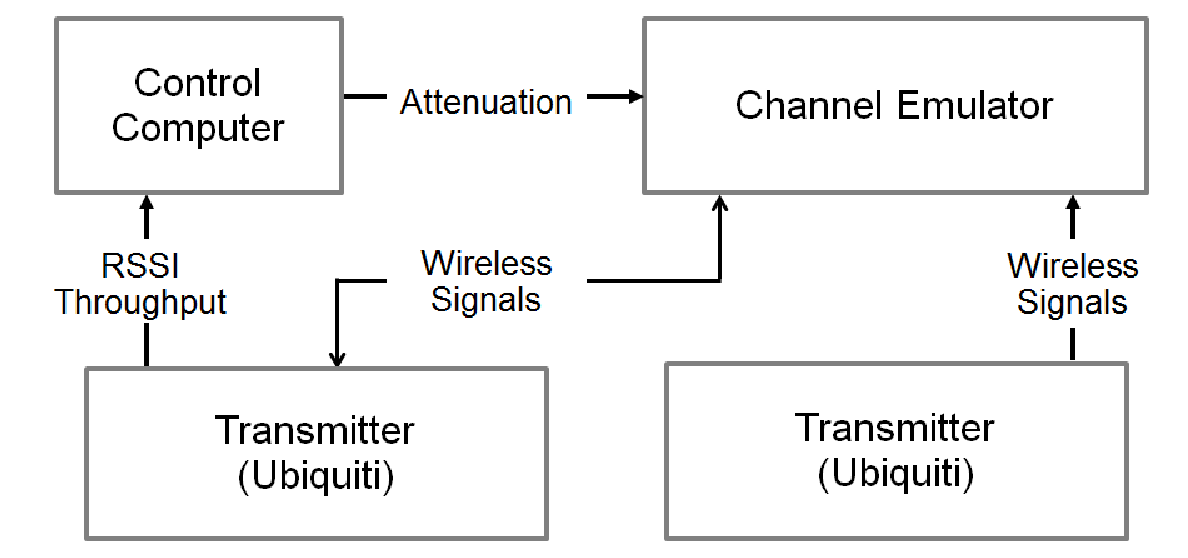
\includegraphics[width=65mm]{figure/emulator2}
\vspace{-0.1in}
\caption{Experimental setup for channel emulator.}
\label{fig:in-door experiment}
%\vspace{-0.1in}
\end{figure}

%\subsection{Signal Level Context-aware information}
\subsection{Experimental Design for In-field Data Collection}
\label{subsec:insitu}
We now describe the in-field experimental design to obtain a data set for
evaluating our multiband algorithms. Two Gateworks boards, each containing
the aforementioned four radios are installed on two cars.  One node is always
the receiver and at a fixed location. The other node is always the 
transmitter and traverses
around the block of a public park as shown in Figure~\ref{fig:infield},
one loop of which will be used as a unit of training in the next section.
 
\begin{figure}
%\vspace{-0.1in}
\centering
\includegraphics[width=75mm]{figure/infield}
\vspace{-0.1in}
\caption{In-field Experiment Setup}
\label{fig:infield}
\vspace{-0.1in}
\end{figure}

During each loop, the transmitter sends a fully-backlogged UDP flow
using {\it iperf} over each of the four radios simultaneously.  To
focus on band selection, we disable autorate and use a fixed data rate
of 6 Mbps. The receiver continually performs a {\it tcpdump} of all
received 802.11 packets~\cite{jacobson1989tcpdump}. Additionally, a
QH 400 Quad Ridge Horn antenna (shown in Figure~\ref{fig:infield}) is 
connected to a Rhode \& Schwarz FSH8 mobile spectrum analyzer at the 
receiver's location to monitor spectral activity. Then, based on the 
time stamps, 802.11 packets can be removed from the spectral trace 
so that only non-802.11 interference will contribute to $P_N^N$ for 
our algorithms.

\begin{figure}
\vspace{-0.1in}
\centering
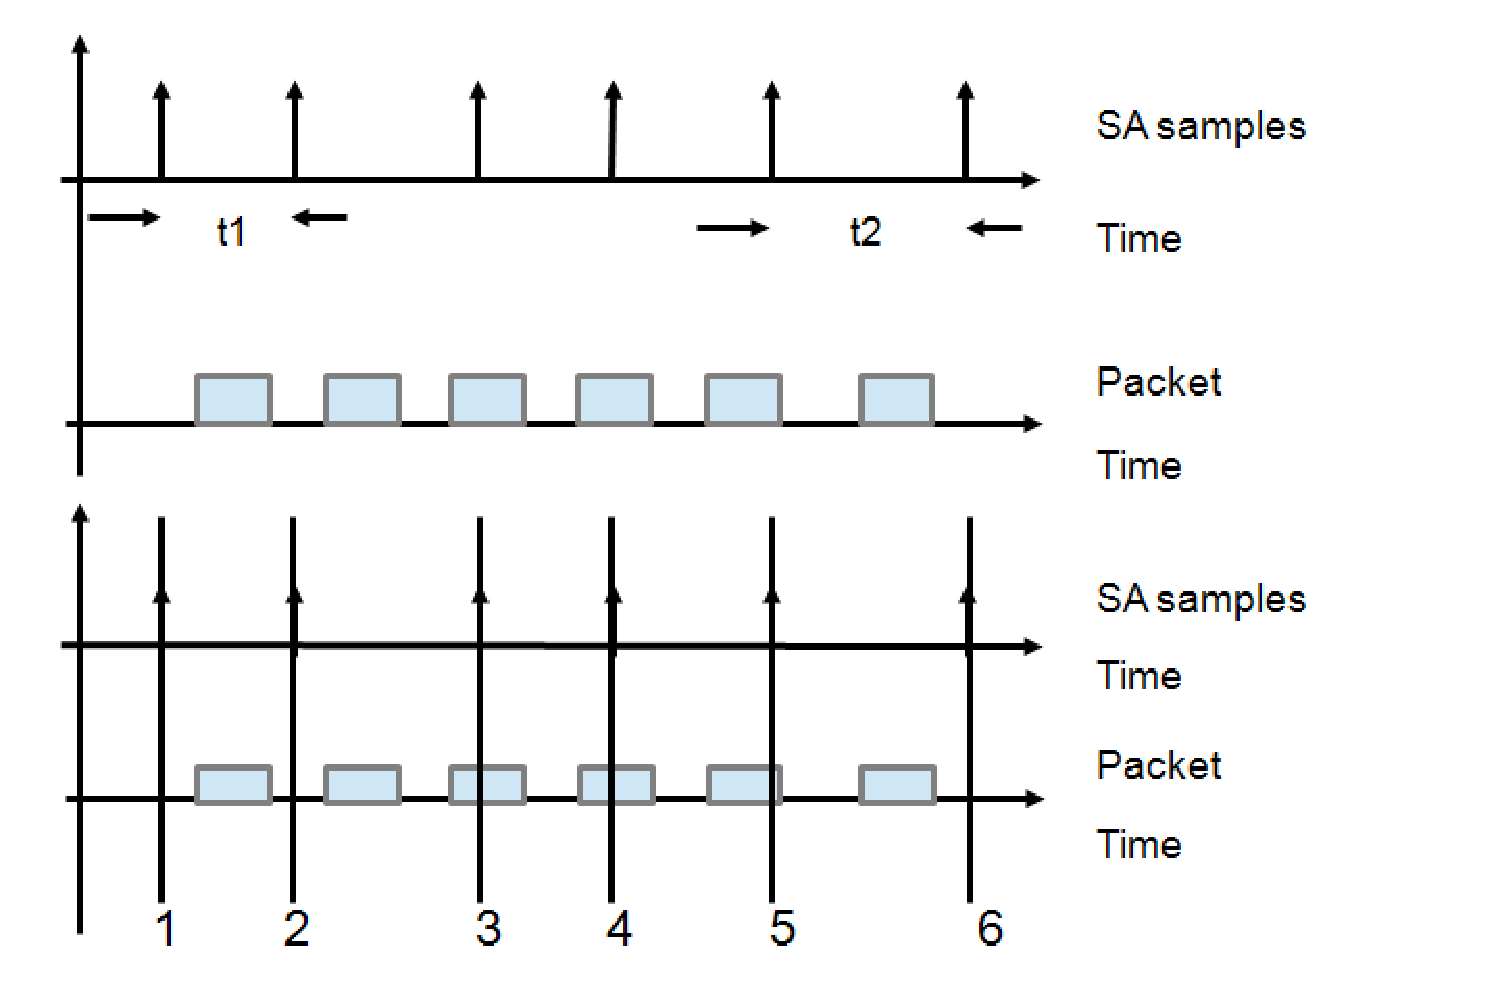
\includegraphics[width=65mm]{figure/sa_process}
\vspace{-0.1in}
\caption{Spectrum Analyzer Data Processing}
\label{fig:sa_process}
%\vspace{-0.1in}
\end{figure}

Figure~\ref{fig:sa_process} shows how we find the value of the
non-802.11 interference, $P_N^N$. We delete the spectrum analyzer
(SA) samples which overlap in time with the dumped 802.11 packets,
such as packet 3, 4, and 5 shown. Then, the reported interference value
will not contain received power from 802.11 packets which have already
been considered in the busy time, $B$.

The in-field data is processed offline where data from all instruments
involved is synchronized based on the GPS time stamps of each. 
As discussed in~\ref{subsec:ichannel}, the throughput of each radio
is normalized based upon the emulator experiment to account for any
manufacturing differences.


\section{Data Process}
\label{sec:experiment}

Fixme


%Detail may not useful
Parsing script
In our experiments, we are constantly collecting large amounts of data, including the received signal level, current location, velocity, and time of day. Working with the memory-limited Gateworks boards, it became necessary to implement a solution to collect large amounts of data without exhausting the available memory space on the boards. Thus, we compiled a script to parse an undetermined number of data files containing the raw data collected from the ongoing experiments. Utilizing the Perl programming language, which the Gateworks boards are capable of running, the script scans every file in a directory we specify and parses them, looking specifically for signal level, lat/long location, velocity, and time data recorded from the experiments. Upon finding this information, the script reformats the data by placing it into a .csv file. Additionally, using the location data, the script calculates the  distance between the transmitting and receiving boards and adds this information to the .csv file. Upon parsing the data, the raw experimental data files can simply be delete from memory, freeing up space for the data of subsequent experiments.

Activity monitor script
For in-situ experiments, the need became apparent to track the number of new incoming packets and compare it with the number of previously received packets. Additionally, this needed to be done for each of the four wireless radios on the board. In doing this, we identify the most efficient frequency band to transmit data. To implement this system, a script was needed to run efficiently in the background while experiments were taking place. To achieve this, we wrote a bash shell script to run directly on the board without relying on any higher level programming language that could potentially cause greater performance overhead. As a result, the script only consumes one to two percent of CPU resource. The script begins by examining the received bytes across each radio for a length of 30 seconds and placing the bytes received each second on a new line in a file. Upon the completion of the 30 second buffering time period, the next second of received bytes on each radio is read and compared with the last 30 seconds of received data. This ratio of the most recent received data to old received data is then calculated and written to four files, one for each radio, for its subsequent use in selecting which radio to transmit/receive from.


%\section{Related Work}
\label{sec:related}

Cognitive Radio could be a powerful tool for the utility of the Spectrum Opportunity~\cite{haykin2005cognitive}.
Analog TV bands will be released for wireless communication brings opportunity to combine current wireless bands and new available bands for performance improvement employing Cognitive Radio methods~\cite{MOAR}. 


%Related research
A bunch of work has been done on radio-scene analysis and channel identification for utility of channel adaptation dating back to Simon Haykin~\cite{haykin2005cognitive}.
Some work of Multi-bands/Multi-channels in
cognitive radios focus on optimize performance, such as avoiding frequency diversity~\cite{rahul2009frequency}. 
In~\cite{OAR} an opportunistic algorithm is introduced to balance the cost of spectrum sensing, channel switching and the gain of these activities.


%Our work
Our work is motivated by prospective releasing band used for TV now and exploit the comparison across all the available bands in the future. 
It is an extension of multi-channel adaptation. 
Most of the published research focus on the stopping rules of spectrum sensing~\cite{sabharwal2007opportunistic, OAR}. In contrast, we use the data and framework to classify the performance across different bands based on the parameters we get from the context information.
%{\bf .} 


\section{Summary}
\label{sec:vncsummary}


In this chapter, we investigated multiband adaptation to leverage the propagation and context for vehicular applications. 
We did so by proposing two machine-learning-based schemes and compared their
performance against two baseline schemes.
In our experimental analysis, we evaluated the performance of these algorithms 
in the field on an off-the-shelf platform.
Experimental results demonstrate that the proposed algorithms can 
achieve up to 49.3\% greater throughput than the baseline algorithms
with an accuracy up to 65\%. In future work, we will study the impact that
multiple diverse environments have on the training as well as evaluate
the optimal use of multiple, diverse radios in unison.
%Since mobile networks have limited
%energy and training in multiple environment has not been investigated, in future work we plan to examine the influence of diverse environment and energy efficiency of
%the simultaneous use of multiple, diverse radios.

%
\section{Acknowledgments}

This work was supported by in part by NSF grants 
CNS-0958436, CNS-1040429, and CNS-1150215 and
Toyota InfoTechnology Center, U.S.A. Inc.




\bibliographystyle{IEEEtran}

\bibliography{multiband}

\end{document}
%This is never printed
